\documentclass[12pt]{article}
\usepackage[english]{babel}
\usepackage[utf8x]{inputenc}
\usepackage[T1]{fontenc}
\usepackage{scribe}
\usepackage{listings}
\usepackage{tcolorbox}

\Scribe{Students and TA Team}
\Lecturer{Abir De}
\LectureNumber{5}
\LectureDate{22nd August 2022}
\LectureTitle{Classification and Ranking Problem}

\lstset{style=mystyle}

\begin{document}
	\MakeScribeTop

%#############################################################
%#############################################################
%#############################################################
%#############################################################

In this lecture, we begin by trying to make our classification model more robust to noise, after which we move on to modelling ranking problems

\section{Introduction}

Given data in the form of $(x_i,y_i)$ (i.e. measurement features and label pairs) where $x_i\in \mathbb{R}^d$ and $ y\in\{-1,1\}$ for all $i\in\{1,2,\dots,D\}$ we want to construct an estimator $H: \mathbb{R}^d \rightarrow \{-1,1\}$ that makes predictions as $y^{\textrm{pred}}_i = H(x_i)$. The way to go is to look at a particular class of functions for $H$ and obtain the best parameters in that family of estimators. But before that, choosing that family is also important. We discuss the case when $H$ is linear in $x_i$ (in a sense). 
\\\\
Practically, we would divide the entire dataset into a training set and a validation set and it is to be noted that the following discussion is done only with respect to this training subset of the data. But for simplicity we still denote the set as the same $\{1,2,\dots,D\}$ since it doesn't change the discussion.

\section{Linear estimators}
Say first we want to find an optimal $H$ from the family of constant functions $H(x_i) = c$. The $c$ that is most optimal is the one that minimizes the particular loss function:
\begin{align}
    L = \sum_{i=1}^{D}\mathbb{I}\left(H(x_i) \neq y_i\right) && \textrm{where } \bigg\{ \substack{\mathbb{I}(\textrm{true}) = 1 \\ \mathbb{I}(\textrm{false}) = 0}
\end{align}
$c_{\textrm{optimal}}$ is $\pm 1$ according to which is bigger: the number of $+1$ labels ($\eta_+$) or the number of $-1$ labels ($\eta_-$) so that it matches the most values from $y_i$. Here $L_{\textrm{min}}$ (minimum loss) will be $ \min(\eta_+, \eta_-)$.
\\\\
Coming to linear estimators, suppose instead that we want $H(x_i) = \textrm{sgn} (\omega^{\top} x_i + b)$ (assuming, for now, that we don't encounter $\textrm{sgn}(0)$. $\textrm{sgn}$ is signum function). This function is representative of assigning a score for each $x_i$ (by a linear operation $\omega^{\top}x_i + b$) and classifying $x_i$ according as if this score is positive or negative. We can try to minimise the same loss as before:
\begin{align}
    L = \sum_{i=1}^{D}\mathbb{I}\left(H(x_i) \neq y_i\right)
\end{align}
but the objective function to minimise here is not continuous. We can try to come up with a different, but continuous, loss function that is representative of the same needs. 
\\\\
Say true label (i.e. $y_i$) is $+1$. Then a desirable $x_i$ will have $\omega^{\top}x_i + b > 0$ (positive score). Instead of assigning a fixed loss of $1$ for the undesirable case of $\omega^{\top}x_i + b < 0$ (negative score), which is making the loss function discontinuous, a continuous loss metric can be $l(x_i) = \text{max}(0,-(\omega^{\top}x_i + b))$. Similarly if label was $-1$ we would desire a negative score and a continuous loss for that case may be as $l(x_i) = \text{max}(0,\omega^{\top}x_i + b)$. All in all our new loss function to minimise is:
\begin{align}
    L = \sum_{i=1}^{D}\textrm{max}\left(0, -y_i(\omega^{\top}x_i + b)\right)
\end{align}
From now we will shorten $\textrm{max}(0, \cdot)$ to $(\cdot)_+$. This function is sometimes referred to as `ReLU' (Rectified Linear Unit).

Note that the loss term is still zero when, for example, $\textrm{signum}(\omega^{\top}x_i + b) = y_i$ which is in line with $\mathbb{I}(H(x_i) \neq y_i)$. With alternate loss metrics to minimise, we are still rewarding the same functions but are just penalising them differently. These `alternate' loss functions are called surrogate loss functions when they are used instead of $\mathbb{I}(H(x_i)\neq y_i)$

\section{Accounting for noise in measurements}
So far, the classification method for our predictions say that:
\begin{align}
    y_i^{\textrm{pred}} = \begin{cases}
        +1 & \omega^{\top}x_i + b > 0\\
        -1 & \omega^{\top}x_i + b < 0
    \end{cases}
\end{align}
But this way our predicted values can change from $1$ to $-1$ if a small amount of noise in $x_i$ causes $\omega^{\top}x_i + b$ to go from positive to negative. A common way to address this apparent discontinuity in our classification is to instead do this:
\begin{align}
    y_i^{\textrm{pred}} = \begin{cases}
        +1 & \omega^{\top}x_i + b > 1\\
        -1 & \omega^{\top}x_i + b < -1
    \end{cases}
\end{align}
This is `making sure' that the score $\omega^{\top}x_i + b$ is `positive enough' before saying $y_i^{\textrm{pred}} = +1$, for example. We could have replaced $1,-1$ with some $a,-a$ as well but it is an equivalent problem since we are finding optimal $\omega,b$ and so will just divide by $a$. Again we are assuming, for now, that $\omega^{\top}x_i + b$ does not lie between $1$ and $-1$. If it is, it's only an issue for the actual classification since our continuous loss functions do not `break' for any $x_i$ this way. 
\begin{tcolorbox}
The condition assumed earlier, that $\omega^{\top}x_i + b$ does not lie between $1$ and $-1$ can occur only when the convex hull determined by all the points with $y=1$ and the convex hull determined by the points with $y=-1$ do not intersect (A convex hull of a set of points is defined as the smallest area convex polygon that encloses all the points). In this case, an ML model is not really needed since a deterministic construction of the convex hull would give well enough results. It is when there are ambiguous cases that ML truly shines.
\end{tcolorbox}
Anyway, we will now accordingly need to modify our Loss function from before. We use the same reasoning to replace the constant loss of 1 in the undesirable case to a continuous extension of the desirable case. Say the score ($z$) is $z = \omega^{\top}x_i + b$. If $y_i = +1$ then loss is modelled as $(0,1-z)_+$ and if $y_i = -1$ then loss is $(0,1+z)_+$. Here we want to count some loss even if $z$ and $y_i$ have the same sign but $|z|<1$ (correct prediction, but not by enough margin).
\\\\
We will therefore write:
\begin{align}
    L = \sum_{i=1}^{D}\left( 1-y_i(\omega^{\top}x_i + b)\right)_+
\end{align}

Where $(\cdot)_+ = \textrm{max}(0,x)$. This type of loss (of the form $(1-yz)_+$ where $z$ is the score and $y$ is the label) is called a Hinge loss function and is the basis for Support vector machines (a.k.a SVM).

\section{Likelihood Estimator for Classification Problems}

Sigmoid function is very commonly used in ML solution formulations. It is defined as :-\\
\begin{align*}
    S(x) &= \frac{1}{1+e^{-x}}
\end{align*}
We have already seen ways to define the loss metric for classification problems. Here, we define a estimator of the probability of getting the given estimates from our ML model, that forms the basis of the Maximum Likelihood Estimator (MLE).\\
In order to use MLE, we have to make two important assumptions, which are typically referred to together as the i.i.d. assumption. These assumptions state that:
\begin{enumerate}
    \item Data must be independently distributed.
    \item Data must be identically distributed.
\end{enumerate}

Our initial loss function was defined as :-

\begin{align*}
    L &= \sum_{i \in D} \mathbb{I}(\mathbf{H}(x_i)\neq y_i)
\end{align*}

Since we can scale the loss function by any factor, let us divide it by $|D|$. So, now we have :-
\begin{align*}
    L &= \frac{1}{|D|}\sum_{i \in D} \mathbb{I}(\mathbf{H}(x_i)\neq y_i)\\
    &= \mathbb{E}\left[\mathbb{I}(\mathbf{H}(x)\neq y)\right]\\
    &= Pr(\mathbf{H}(x)\neq y)
\end{align*}

The last step follows because we are taking expectation of the indicator function.\\

The value associated with a given data sample is given by the same linear transformation as before ($\vec{w}^{T}\vec{x}+b$). To get the probability, we apply the Sigmoid function to this value to get:-

\begin{align*}
    Pr(y=1|x) &= \frac{1}{1+e^{-(\vec{w}^{T}\vec{x}+b)}}\\
    Pr(y=-1|x) &= \frac{1}{1+e^{(\vec{w}^{T}\vec{x}+b)}}\\
    Pr(y|x) &= \frac{1}{1+e^{-y(\vec{w}^{T}\vec{x}+b)}}
\end{align*}

Since, the data samples can be considered to be independent of each other, it makes intuitive sense to compute the product of the probabilities so obtained.\\

\begin{align*}
    Pr(Y|X) &= \prod_{i \in D}Pr(y_i|x_i)\\
\end{align*}

This probability tells us the likelihood of getting the measurements we have using the linear transformation tuple $(\vec{w},b)$. The higher this probability, the better. Equivalently; the lower the negative log likelihood, the better.
\begin{align}
    -\ln Pr(Y|X) &= \sum_{i \in D}-\ln Pr(y_i|x_i) \\
    &= \sum_{i \in D}\ln \left(1+e^{-y_i(\vec{w}^{T}\vec{x_i}+b)}\right)
\end{align}
This may be taken as yet another loss metric to be minimised. In fact, the function $\ln (1+e^z)$ happens to be similar to $(z)_+$ in shape (here $z = -y_i(\vec{w}^{T}\vec{x_i}+b)$) with the added benefit of being differentiable at $0$. This supports the notion that the earlier formulation of loss function using $(z)_+$ is probably right.

\begin{figure}[h]
    \centering
    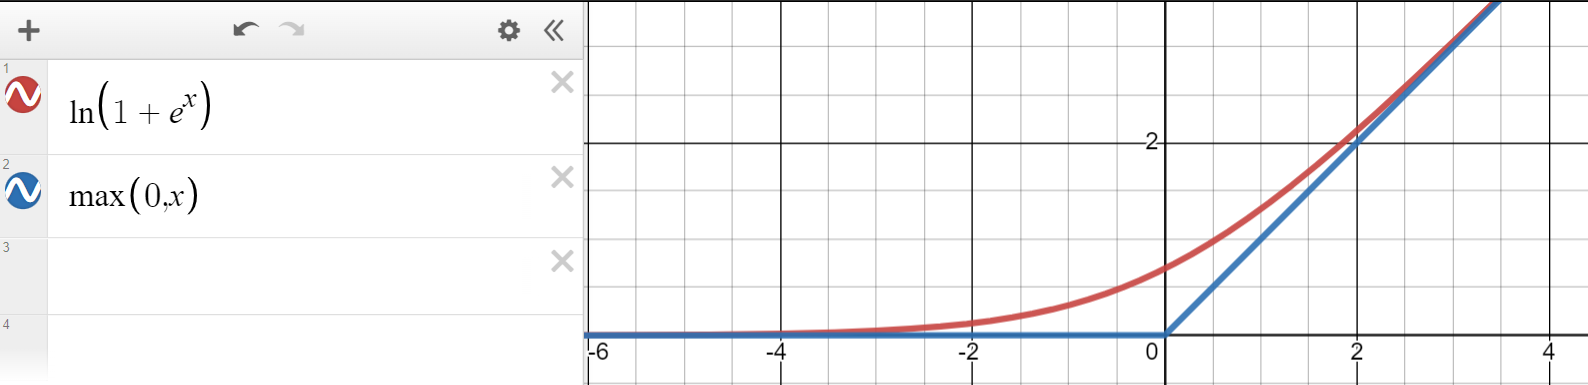
\includegraphics[width=400pt]{graph.png}
    \caption{Comparing $(x)_+$ and $\ln (1+e^x)$}
\end{figure}

\section{Example Problem for finding Loss Function}

Imagine a website (Amazon, if you will) where products have 3 attributes :-

\begin{enumerate}
    \item price (p)
    \item quality (q)
    \item brand (b)
\end{enumerate}

We have to classify the products as 1 (products customer would be willing to buy) and $-1$ (products customer would not be willing to buy). We have the following condition to determine the value of $y$ :-

\begin{align*}
y &=\begin{cases} 
      1 & \vec{w_p}^{T}\vec{P}+\vec{w_q}^{T}\vec{Q}> 1 \\
      1 & \vec{w_p}^{T}\vec{P}+\vec{w_q}^{T}\vec{Q} < -1 \text{ and } \vec{w_b}^{T}\vec{B} \geq 0  \\
      -1 & \vec{w_p}^{T}\vec{P}+\vec{w_q}^{T}\vec{Q} <-1 \text{ and } \vec{w_b}^{T}\vec{B} < 0
   \end{cases}
\end{align*}

We take the loss function as :-

\begin{align*}
    loss = \sum_{i \in D}{max(0,\vec{w_b}\vec{B_i}\cdot min(\vec{w_p}^{T}\vec{P_i}+\vec{w_q}^{T}\vec{Q_i},0)y- max(\vec{w_p}^{T}\vec{P_i}+\vec{w_q}^{T}\vec{Q_i},0)y)}
\end{align*}

Here, if $\vec{w_p}^{T}\vec{P_i}+\vec{w_q}^{T}\vec{Q_i} > 0$, then $loss = 0$ if $y = 1$, and positive if $y=-1$. If $\vec{w_p}^{T}\vec{P_i}+\vec{w_q}^{T}\vec{Q_i} < 0$, then if $\vec{w_b}^{T}\vec{B} > 0$, $loss=0$ if $y=1$ and positive if $y=-1$. Finally if $\vec{w_p}^{T}\vec{P_i}+\vec{w_q}^{T}\vec{Q_i} < 0$, and if $\vec{w_b}^{T}\vec{B} < 0$, $loss=0$ if $y=-1$ and positive if $y=1$. This agrees with the conditions given to us in the beginning and hence, the function is an appropriate loss function.\\

\section{Ranking Problem}

Up till now, we have been dealing with classification problems where we had to put labels on a specific data element. Now, we make our problem a bit more complex.\\

This problem is inspired by how search engines rank pages based on queries given by the user.\\

We have been given a set of pages $\{P_i\}$. Our dataset consists of tuples of queries and orderings of the form $\{Q_i,O_i\}$ where $O_i$ is an ordering of the pages in $P$. The aim is to find the page ranking for queries $Q^{\text{new}}_i$, that are previously unseen.\\

The first step to solving this problem is to design an appropriate loss function.\\

We define the similarity between a query $q$ and a page $c$ as a feature vector $\vec{x_{qc}}$. If we use the linear weight $\vec{w}$ and bias $b$, then we can associate with each page (for a specific query) the value given by $\vec{w}^{T} \vec{x_{qc}} +b$.\\

Since we want a ranking here, we want a loss function such that :-

\begin{enumerate}
    \item If $\vec{w}^{T} \vec{x_{qc_1}} +b>\vec{w}^{T} \vec{x_{qc_2}} +b$ and $r_{c_1}<r_{c_2}$ (i.e. $c_1$ comes before $c_2$), then we want the loss to be 0 or close to 0.
    \item If $\vec{w}^{T} \vec{x_{qc_1}} +b>\vec{w}^{T} \vec{x_{q{c_2}}} +b$ and $r_{c_1}>r_{c_2}$ (i.e. $c_1$ comes after $c_2$), we want the loss to be positive, preferably a monotonic function of the difference between the ranks and difference between the values.
\end{enumerate}

Here, we find an appropriate function :-

\begin{align*}
    \sum_{c_1,c_2 \in P} max(1+(r_{c_1}-r_{c_2})(\vec{w}^{T}(\vec{x_{qc_1}}-\vec{x_{qc_2}})),0)
\end{align*}

In case 1, the first argument of the $max$ function becomes negative, and so it gives a 0 loss. In case 2, the first argument of the $max$ becomes positive and the greater the difference in the ranks and values, the greater is the value of the loss.\\

We have added 1 to the first argument because we need to separate the values by a sizeable margin to reduce ambiguity and the effect of noise on the model. This is similar to the logic used before in the previous model.\\
%%%%%%%%%%% If you don't have citations then comment the lines below:
%
% \bibliographystyle{abbrv}           % if you need a bibliography
% \bibliography{mybib}                % assuming yours is named mybib.bib


%%%%%%%%%%% end of doc
\end{document}